\documentclass[12]{amsart}

\usepackage{amsmath}
\usepackage{amsthm}
\usepackage{tikz}
\usepackage{tikz-3dplot}
\usetikzlibrary{calc,patterns,angles,quotes,positioning}


\theoremstyle{definition}
\newtheorem{theorem}{Theorem}
\newtheorem{claim}[theorem]{Claim}
\newtheorem{definition}[theorem]{Definition}
\newtheorem{corollary}[theorem]{Corollary}

\newcommand{\AxisRotator}[1][rotate=0]{\tikz[x=0.25cm,y=0.60cm,-stealth,#1] \draw (0,0) arc (-150:150:1 and 1);}
\newcommand{\AxisRotatorUnder}[1][rotate=0]{\tikz[x=0.25cm,y=0.60cm,-stealth,#1]
  \draw (0,0) arc (150:-150:1 and 1);}


\begin{document}
    \title{Cat Flipping}
    \author{Arden, Sean, and Will}
    \maketitle
    
    \section{Moment of Inertia of the Cat}
    We model a falling cat with two cylinders $A$ and $B$ connected by a spherical joint (which we assume to be massless) with $A$ and $B$ separated by angle $\theta$.

    \begin{claim}
        About the center of mass, the $y$ axis of the cat is principle. Further, we can write $\vec{L} = (2I_{yy})\omega_y\hat{y}$. For an $I_{yy}$ dependent on the geometry of the cylinders and $\theta$.
    \end{claim}
    \begin{proof}
        Let the moment of inertia tensors of cylinders $A$ and $B$ about the center of mass of the cat as a whole be denoted $I_A$ and $I_B$. Recall the definition of the moment of inertia tensor:        
        \begin{equation*}
            I =
            \begin{pmatrix}
                \sum(y^2+z^2) & \sum xy       & \sum xz     \\
                \sum yx      & \sum(x^2+z^2) & \sum yz      \\
                \sum zx      & \sum zy       & \sum(x^2+y^2)
            \end{pmatrix}
        \end{equation*}
        Then, by the reflectional symmetry of bodies $A$ and $B$, the calculations for $I_A$ and $I_B$ are identical except for the replacement of $y$ by $-y$. So, we can safely write
        \begin{equation*}
            I_A = 
            \begin{pmatrix}
                I_{xx} & I_{xy} & I_{xz} \\
                I_{yx} & I_{yy} & I_{yz} \\
                I_{zx} & I_{zy} & I_{zz}
            \end{pmatrix} \text{ and }
            I_B = 
            \begin{pmatrix}
                I_{xx} & -I_{xy} & I_{xz} \\
                -I_{yx} & I_{yy} & -I_{yz} \\
                I_{zx} & -I_{zy} & I_{zz}
            \end{pmatrix},
        \end{equation*}
        And so the moment of inertia tensor $I$ of the cat as a whole is of the form
    \begin{equation*}
        I = I_A + I_B = 
            \begin{pmatrix}
                2I_{xx} & 0       & 2I_{xz} \\
                0       & 2I_{yy} & 0 \\
                2I_{zx} & 0       & 2I_{zz}
            \end{pmatrix}
    \end{equation*}
    Then $\vec{y}$ is a clear eigenvector of $I$ confirming that the $y$ axis is a principle axis. 
    \label{claim:principle}
    \end{proof}    
    Note that the above argument can be generalized to any two bodies with reflectional symmetry through the $x,y$ plane.
\begin{claim}
    The $I_{yy}$ in claim \ref{claim:principle} can be written $I_{y'y'} \cos^2(\theta/2) + I_{z'z'} \sin^2(\theta/2)$ where $I_{y'y'}$ and $I_{z'z'}$ are the moment of inertia elements corresponding to the principle axes.
\end{claim}
\begin{proof}
    Let $x',y',z'$ denote the principle axes of cylinder $A$ about the center of mass with $z'$ going down the length of the cylinder, $x'$ parallel to $x$, and $y'$ in the corresponding location for a right-handed orthogonal coordinate system. Then, with this coordinate system corresponding to the principle axes, we can write the moment of inertia tenor $I_A'$ of cylinder $A$ about the center of mass of $A$.
    \begin{equation*}
        I_A = 
        \begin{pmatrix}
                I_{x'x'} & 0 & 0 \\
                0 & I_{y'y'} & 0 \\
                0 & 0 & I_{z'z'}
        \end{pmatrix}
    \end{equation*}
    Now, we adjust to the $x,y,z$ coordinate system established above and solve for $I_{yy}$. Note $\hat{y}$ is given by $(0, \cos(\theta/2), \sin(\theta/2))$ in $x',y',z'$ coordinates. Thus by adjusting coordinates we have
    \begin{align*}
        I_{yy} &=
        \begin{pmatrix}
            0 & \cos(\theta/2) & \sin(\theta/2)
        \end{pmatrix}
        \begin{pmatrix}
            I_{x'x'} & 0 & 0 \\
            0 & I_{y'y'} & 0 \\
            0 & 0 & I_{z'z'}
        \end{pmatrix}
        \begin{pmatrix}
            0 \\ \cos(\theta/2) \\ \sin(\theta/2)
        \end{pmatrix}\\
        &= I_{y'y'} \cos^2(\theta/2) + I_{z'z'} \sin^2(\theta/2)
    \end{align*}
    The above gives the value of $I_{yy}$ about the center of mass of $A$, but the center of mass of the cat as a whole shares identical $x$ and $z$ values. So, by $I_{yy} = \sum x^2+z^2$, the value of $I_{yy}$ holds about the center of mass the cat.
    
\end{proof}
Again, note the above argument is generalizable given the principle axes.

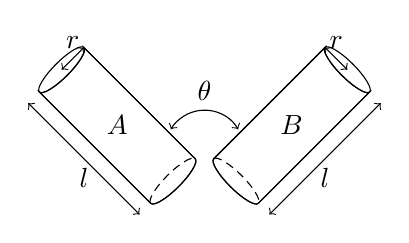
\begin{tikzpicture}[scale=1, transform shape]
  \begin{scope}[shift={(-0.4,0.0)}, rotate=45]
    \draw (0.4,0) -- (0.4,2.0) arc (360:180:0.4cm and 0.1cm) -- (-0.4,0) arc
    (180:360:0.4cm and 0.1cm);
    \draw (-0.4,2.0) -- (-0.4,0) arc (180:360:0.4cm and 0.1cm) -- (0.4,2.0) ++
    (-0.4,0) circle (0.4cm and 0.1cm);
    \draw[densely dashed] (-0.4,0) arc (180:0:0.4cm and 0.1cm);

    \draw[<->] (-0.6,0.0) -- node[below,midway,rotate=-45] {$l$} (-0.6, 2.0);
    \draw[<->] (0.0,2.0) -- node[above,midway,rotate=-45] {$r$} (0.4,2.0);

    \node[rotate=-45] at (0.0, 1.0) {$A$};
  \end{scope}
  \begin{scope}[shift={(0.4,0.0)}, rotate=-45]
    \draw (0.4,0) -- (0.4,2.0) arc (360:180:0.4cm and 0.1cm) -- (-0.4,0) arc
    (180:360:0.4cm and 0.1cm);
    \draw (-0.4,2.0) -- (-0.4,0) arc (180:360:0.4cm and 0.1cm) -- (0.4,2.0) ++
    (-0.4,0) circle (0.4cm and 0.1cm);
    \draw[densely dashed] (-0.4,0) arc (180:0:0.4cm and 0.1cm);

    \draw[<->] (0.6,0.0) -- node[below,midway,rotate=45] {$l$} (0.6, 2.0);
    \draw[<->] (-0.0,2.0) -- node[above,midway,rotate=45] {$r$} (-0.4,2.0);

    \node[rotate=45] at (0.0, 1.0) {$B$};
  \end{scope}
  \coordinate (A) at (-1,1);
  \coordinate (B) at (1,1);
  \coordinate (O) at (0,0.4);
  \pic[draw, <->, "$\theta$",angle eccentricity=1.5]{angle=B--O--A};
\end{tikzpicture}


\end{document}
